\documentclass[a4paper,10pt]{article}

\usepackage{eripage}
\usepackage[dvips]{graphicx}
%\usepackage{garamond}

\Document{System description}
\Prepared{ETH/RZX J\'anos Zolt\'an Szab\'o}
\Tel{+36 1 437 7635}
\Date{2007-06-04}
\Rev{PA17}
\Documentno{ }
\Checked{ }
\Approved{APPROVED}
%\Yourdate{4th November 2000}
\Ref{ }

\usepackage{longtable}

\begin{document}

\pagestyle{erifull} % Chose from erismall, eriplain, erifull

\Title{Architecture for Parallel and Distributed \\
Execution of TTCN-3 Test Suites}

\begin{abstract}
This document describes a generic framework, which enables the parallel and distributed execution of TTCN-3 test suites with more than one test component. The document covers the implementation of all TTCN-3 operations related to parallel test execution (component management, synchronization, internal communication).
\end{abstract}

\section*{Revision History}
\begin{tabular}{|c|c|c|l|}
\hline
Date & Signature & Version & Comment \\
\hline
2001-03-14 & TMPJSZ & PA1 & First draft. \\
\hline
2001-03-21 & TMPJSZ & PA2 & Message types were added. \\
\hline
2001-05-02 & TMPJSZ & PA3 & Minor corrections. \\
\hline
2001-05-10 & TMPJSZ & PA4 & Format of message DONE changed. \\
\hline
2001-06-06 & TMPJSZ & PA5 & Missing message DISCONNECT\_ACK added. \\
\hline
2001-06-08 & TMPJSZ & PA6 & Port connection mechanisms changed. \\
           &        &     & Connectionless communication removed. \\
\hline
2001-06-20 & TMPJSZ & PA7 & Minor changes related to port connections. \\
\hline
2002-09-16 & TMPJSZ & PA8 & General revision. \\
\hline
2003-01-15 & TMPJSZ & PA9 & Minor error corrections. \\
\hline
2003-03-31 & TMPJSZ & PA10 & Minor corrections to be compliant with the new MC. \\
\hline
2003-06-17 & TMPJSZ & PA11 & Added: return type for messages STOPPED and \\
           &        &      & DONE. Removed: message STARTED. \\
\hline
2003-11-24 & TMPJSZ & PA12 & Added: local connection handling New messages: \\
           &        &      & CONNECT\_LOCAL, CONNECTED\_LOCAL, \\
           &        &      & DISCONNECT\_LOCAL, DISCONNECTED\_LOCAL \\
\hline
2005-05-24 & EJNOSZA & PA13 & Added: static test configurations (alive components). \\
\hline
2006-01-20 & EJNOSZA & PA14 & Updated: control protocol between MC and HCs. \\
\hline
2006-01-22 & EMTYFOR & PA15 & Updated: state machine for MC and HC seen by MC. \\
\hline
2006-06-05 & EJNOSZA & PA16 & Added: transport types and error handling for port \\
           &         &      & connections. Updated: state machines for PTCs and \\
           &         &      & port connections. \\
\hline
2007-06-04 & EJNOSZA & PA17 & Added: transmission of component names to \\
           &         &      & remote components. \\
\hline
\end{tabular}

\tableofcontents

\section{Components of the test system}

[figure: SUT and the test system as a cloud]

The components of test execution form two main groups, regardless of their physical distribution: the Test System and System Under Test (SUT). This document deals with the internal structure of Test System only.

The Test System consists of one or more components, whose behaviours are entirely described in a TTCN-3 test suite. Each component runs independently from each other, they can be considered as different processes of the operating system. Every component executes one single thread.

The components can be located on different machines, but there can be more than one component running on the same computer. In this case the scheduling is provided by the scheduler of the operating system.

The components execute binary code, which can be either a part of the TTCN-3 executor system or generated code according to the TTCN-3 test suite. The hardware and/or operating systems of participating computers may be different, but the code to be executed must be the same at the source code level.

The components can communicate with each other using point to point transport connections and by sending or receiving platform independently encoded abstract messages. It is assumed that making reliable, ordered transport connections (e.g. TCP sessions) is possible between any pair of participating computers.

The components form 3 groups according to their functionality:

\subsection{Main Controller (MC)}
Pieces: 1 in the entire test system\\
Source code: static, i.e. written independently from the TTCN-3 test suite \\
Tasks:
\begin{itemize}
\item MC provides an user interface (command line and/or GUI).
\item Maintains connections with all other components. (One connection with each component.)
\item Arranges the creation and starting of MTC upon user request.
\item Deals with tasks that can only be performed with central coordination (e.g. component creation, verdict collection, etc.).
\item Reads the test suite parameters from a configuration file and distributes them to the remote components.
\item Continuously monitors the state of all components and reports that to the user.
\end{itemize}

\subsection{Host Controller (HC)}
Pieces: 1 on each participating computer \\
Source code: (partly) generated from the TTCN-3 test suite \\
Tasks:
\begin{itemize}
\item HC maintains a connection with MC.
\item When a request arrives from MC, it creates a new component (i.e. it copies itself) on its host computer.
\item It receives and sets test suite parameters. The created new components will inherit these values.
\item HC monitors the load on the local computer and reports it to MC if requested.
\end{itemize}

\subsection{Test Component (TC)}
Pieces: 1 for each TTCN-3 test component (either MTC or PTC). \\
Source code: (partly) generated from the TTCN-3 test suite. The same as HC's. \\
Tasks:
\begin{itemize}
\item Each TC maintains a permanent connection wtih MC.
\item It executes the dynamic part of TTCN-3 test suites (control part, test cases, functions).
\item It communicates with SUT according to the test specification.
\item It can communicate with other (local or remote) TCs using direct connections if the TTCN-3 ports of the two components are connected.
\item It processes the messages coming from MC, but it can also initiate communication with MC.
\end{itemize}

\section{Operation areas related to parallel test execution}
This chapter summarizes those TTCN-3 operations, which should be considered when designing the parallel test architecture.

\subsection{Parameter distribution}
Components affected: MC, HCs \\
Related TTCN-3 operations: NONE

\subsection{Component management}
Components affected: MC, HCs, TCs \\
Related TTCN-3 operations:
\begin{itemize}
\item create
\item (component) start
\item (component) stop
\item kill
\item (component) running
\item alive
\item done
\item killed
\end{itemize}

\subsection{Configuration management}
Components affected: MC, TCs \\
Related TTCN-3 operations:
\begin{itemize}
\item connect
\item disconnect
\item map
\item unmap
\end{itemize}

\section{Other important operation areas}

\subsection{Clock synchronization}

Each participating computer uses its own system clock during the test execution. As the TTCN-3 language does not use the absolute time neither distributed time measurements at all, the clocks of different computers do not need to be synchronized to each other or to an external source.

However, TTCN-3 uses relative times, i.e. the time passed between two test events within one test component. This implies, that the real time elapsed between two events must be measured somehow on all participating computers with enough precision.

In order to get repeatable results, the delay jitter of system clocks between any pair of participating computers during the test execution must be smaller than the delay of communication between the two machines.

The synchronized clocks make the evaluation of test logs easier. It is recommended to use any standard tool (e.g. NTP) for clock synchronization, but this is out of scope of the test executor system.

\subsection{Version control}

It is assumed that the source code of all HC and TC components was generated from the same version of all TTCN-3 modules. Otherwise the operation of the distributed test system will be unpredictable.

Since the version control in the most cases (especially when a large number of computers and TTCN-3 modules are affected) can not be ensured automatically, a version control scheme should be introduced.

It is assumed that a single, but unique version string can be generated from the version numbers of each participating TTCN-3 modules. This can be automated by CASE tools.

When a HC is born, it opens a permanent connection to MC. After the connection is established, the new HC must send its version string to MC in a message. Thus MC can compare and eveluate the version strings of HCs on different computers before starting the test execution. If any version conflict persists, MC will disable the user to start test execution.

If the version of all HCs are the same, no problem will occur because TCs run the same binary code as their HC.

\subsection{Collection of log files}

During the test execution each component (including MC and HCs) produces its own log file on the local machine. Sometimes it can be useful if the user can see all log files together. If the clocks of computers are synchronized, the log files can be merged chronologically into a single file. These log collection tasks should be performed by MC.

The collection of logs must be an optional feature, which can be switched off. For example, after a performance test with thousands of TCs, the traffic generated by log collection incudes more data to be transmitted than during the entire test. It is sure that this will take more time than test execution and can collapse the communication network.

\subsection{Error recovery}

The test system must provide mechanisms, which enable the fast and consistent recovery of the whole system from a dynamic test case error detected by any TC.

\section{Management of TTCN-3 component references}

The test system must assign a unique component reference to each TTCN-3 test component. The test components can identify and refer to each other using these component references. The TTCN-3 language does not specify the internal representation of component references, it may be different on each TTCN-3 tool.

These are the requirements for the component references in this test system:

\begin{itemize}

\item Component references shall be single scalar values (e.g. integer numbers) for more efficient handling (storage, comparison, etc.).

\item Component references are always assigned by MC to the new components. This ensures that no duplicate identifiers can occur.

\item Neither the MC nor HCs shall have component references because they are invisible from TTCN-3 test components.

\item The value range of component references shall have a 'null' value (e.g. 0), which shall not refer to an existing TC.

\item The component reference of MTC shall be a pre-defined and well known constant value (e.g. 1). This value shall be returned by built-in operation {\tt mtc}.

\item The component reference the abstract test system shall also be a pre-defined and well known constant value (e.g. 2). This value shall be returned by built-in operation {\tt system}.

\item MC must identify all TCs (even the terminated ones) based on their component references.

\item Each TC must know its own component reference during its entire lifespan. The newly assigned value shall be transmitted by the MC to its parent HC, which will pass that to the newly created TC. This value shall be returned by built-in operation {\tt self}.

\item MC shall return the component reference of the new TC to the TC that requested the creation. The returned value shall be the result of TTCN-3 {\tt create} operation.

\item Component references of terminated TCs shall not be reused, during the execution of the same test case it is forbidden. The value space must be large enough to give unique identifier to each component created during the entire test execution.

\item TCs shall be able to communicate component references between each other transparently. The abstract messages that are sent or received on communication ports may contain component references. This enables the addressing of components that are not in parent-child relation.

\item The TTCN-3 component variables (the type of which is any component type) shall be represented run-time as a store of a component reference.

\end{itemize}

\section{Types of connections between components}

\begin{figure}[!ht]
\begin{center}
{\resizebox*{\columnwidth}{!}{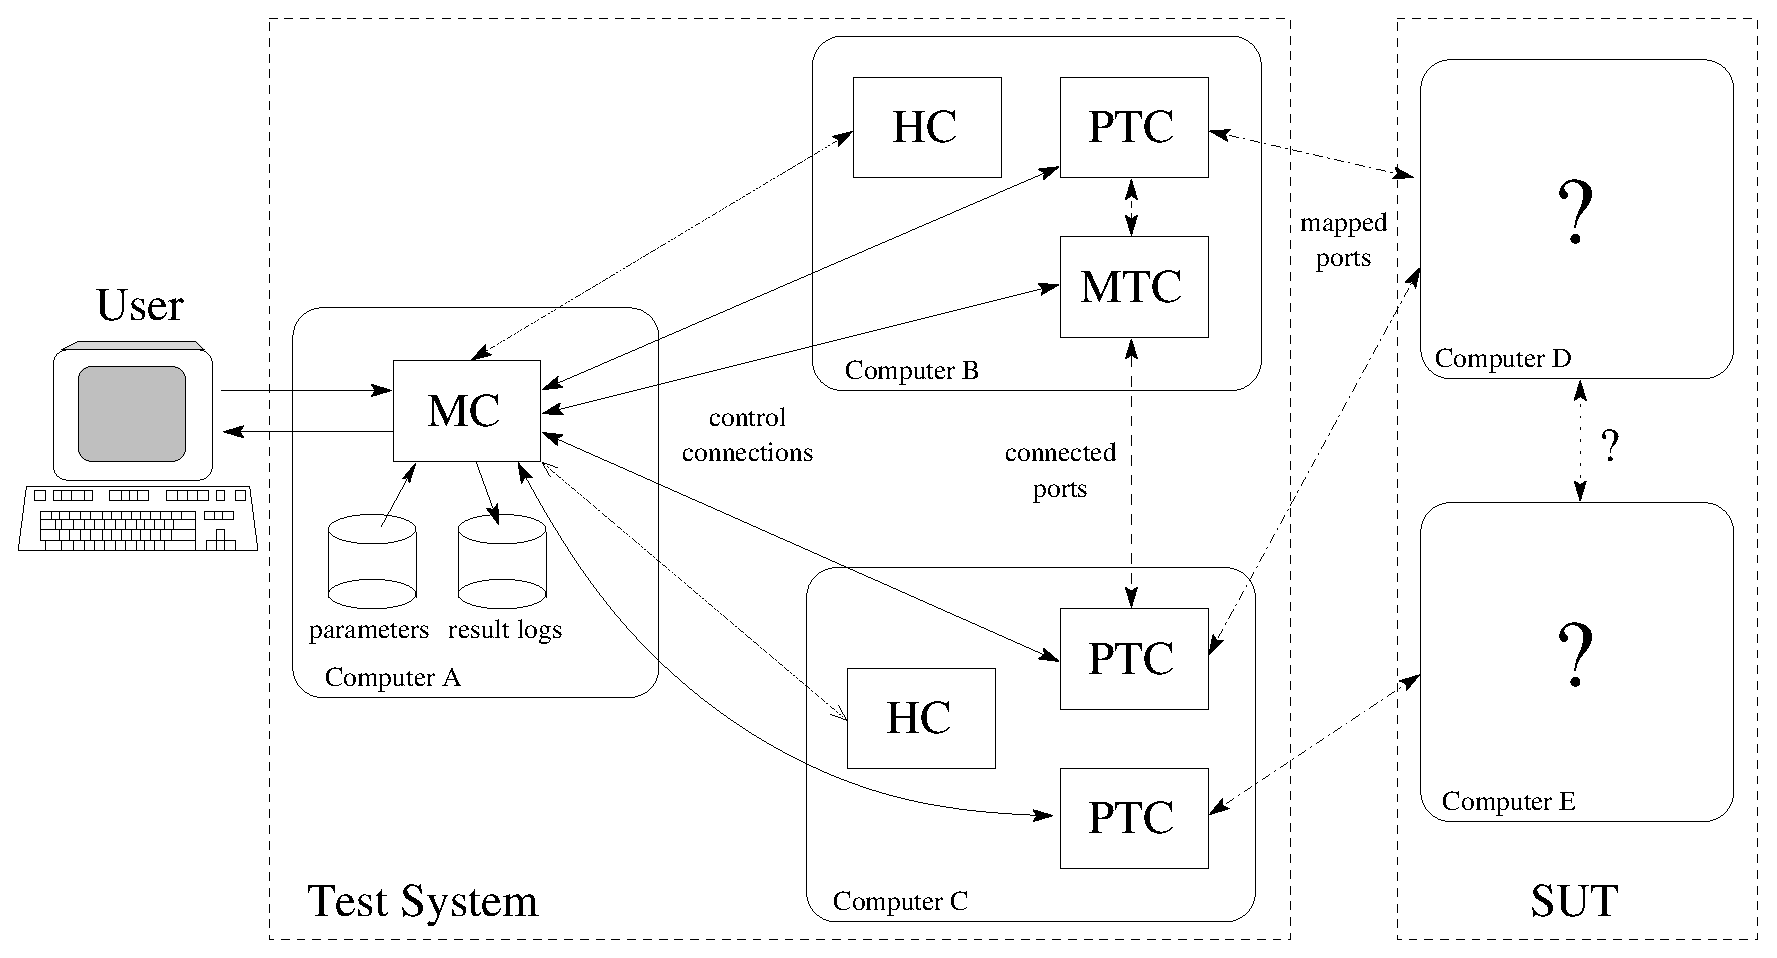
\includegraphics{parallelarch.eps}}}
\end{center}
\caption{\label{figure:parallelarch}A sample configuration with the parallel test architecture}
\end{figure}

\subsection{Connections between MC and HCs}

\emph{Denoted by dashed-dotted lines.}

\subsection{Connections between MC and TCs}

\emph{Denoted by continuous lines.}

\subsubsection{Connection between MC and MTC}

\emph{Denoted by a continuous line.}

As the role of MTC is more complex than other TCs, the communication with MTC uses special messages that are not sent to or received from other TCs.

All messages that can be communicated to 'simple' TCs can also be sent to MTC. It is useful if these common messages...

\subsection{Connection between two connected ports of TCs}

\emph{Denoted by dashed lines.}

\subsection{Connection between the test system and SUT}

\emph{Denoted by dashed-dotted lines.}

These communication channels (including the connection establishment and termination and the communication iteslf) are outside the scope of this document.

The communication with SUT is system dependent, which cannot be done in an uniform way. Hence it is the user's responsibility to perform the physical communication with SUT. To facilitate this, the Test System provides the user with a Test Port API.

\newpage

\section{Implementation of TTCN-3 operations related to parallel test execution}

To be written. [with MSCs]

\begin{figure}[!p]
\begin{center}
{\resizebox*{0.5 \columnwidth}{!}{\includegraphics*[5,280][345,630]{starting_HC.eps}}}
\end{center}
\caption{\label{figure:starting_HC}MSC of starting a HC}
\end{figure}

\begin{figure}[!p]
\begin{center}
{\resizebox*{0.7 \columnwidth}{!}{\includegraphics*[5,300][390,620]{creating_MTC.eps}}}
\end{center}
\caption{\label{figure:creating_MTC}MSC of creating the MTC}
\end{figure}

\begin{figure}[!p]
\begin{center}
{\resizebox*{0.5 \columnwidth}{!}{\includegraphics*[5,190][270,620]{executing_control.eps}}}
\end{center}
\caption{\label{figure:executing_control}MSC of a control part execution}
\end{figure}

\begin{figure}[!p]
\begin{center}
{\resizebox*{0.5 \columnwidth}{!}{\includegraphics*[10,225][265,620]{executing_testcase.eps}}}
\end{center}
\caption{\label{figure:executing_testcase}MSC of a test case execution}
\end{figure}

\begin{figure}[!p]
\begin{center}
{\resizebox*{0.7 \columnwidth}{!}{\includegraphics*[5,345][370,620]{create_op.eps}}}
\end{center}
\caption{\label{figure:create_op}MSC of a create operation}
\end{figure}

\begin{figure}[!p]
\begin{center}
{\resizebox*{0.7 \columnwidth}{!}{\includegraphics*[10,350][340,620]{start_op.eps}}}
\end{center}
\caption{\label{figure:start_op}MSC of a component start operation}
\end{figure}

\begin{figure}[!p]
\begin{center}
{\resizebox*{0.7 \columnwidth}{!}{\includegraphics*[10,400][330,630]{stop_op.eps}}}
\end{center}
\caption{\label{figure:stop_op}MSC of a component stop operation}
\end{figure}

\begin{figure}[!p]
\begin{center}
{\resizebox*{0.5 \columnwidth}{!}{\includegraphics*[10,365][245,620]{running_op.eps}}}
\end{center}
\caption{\label{figure:running_op}MSC of a component running operation}
\end{figure}

\begin{figure}[!p]
\begin{center}
{\resizebox*{0.7 \columnwidth}{!}{\includegraphics*[10,390][310,630]{done_op.eps}}}
\end{center}
\caption{\label{figure:done_op}MSC of a done operation}
\end{figure}

\begin{figure}[!p]
\begin{center}
{\resizebox*{0.8 \columnwidth}{!}{\includegraphics*[10,350][450,625]{connect_op.eps}}}
\end{center}
\caption{\label{figure:connect_op}MSC of a connect operation}
\end{figure}

\begin{figure}[!p]
\begin{center}
{\resizebox*{0.8 \columnwidth}{!}{\includegraphics*[10,390][340,625]{connect_op_local.eps}}}
\end{center}
\caption{\label{figure:connect_op_local}MSC of a local connect operation}
\end{figure}

\begin{figure}[!p]
\begin{center}
{\resizebox*{0.8 \columnwidth}{!}{\includegraphics*[10,320][450,625]{disconnect_op.eps}}}
\end{center}
\caption{\label{figure:disconnect_op}MSC of a disconnect operation}
\end{figure}

\begin{figure}[!p]
\begin{center}
{\resizebox*{0.8 \columnwidth}{!}{\includegraphics*[5,390][350,625]{disconnect_op_local.eps}}}
\end{center}
\caption{\label{figure:disconnect_op_local}MSC of a local disconnect operation}
\end{figure}

\begin{figure}[!p]
\begin{center}
{\resizebox*{0.6 \columnwidth}{!}{\includegraphics*[10,380][310,615]{map_op.eps}}}
\end{center}
\caption{\label{figure:map_op}MSC of a map operation}
\end{figure}

\begin{figure}[!p]
\begin{center}
{\resizebox*{0.6 \columnwidth}{!}{\includegraphics*[10,380][310,615]{unmap_op.eps}}}
\end{center}
\caption{\label{figure:unmap_op}MSC of an unmap operation}
\end{figure}

\begin{figure}[!p]
\begin{center}
{\resizebox*{0.6 \columnwidth}{!}{\includegraphics*[10,460][260,620]{log.eps}}}
\end{center}
\caption{\label{figure:log}MSC of the transferring a log message to MC}
\end{figure}

\begin{figure}[!p]
\begin{center}
{\resizebox*{0.7 \columnwidth}{!}{\includegraphics*[15,385][330,630]{killing_TC.eps}}}
\end{center}
\caption{\label{figure:killing_TC}MSC of killing an uncontrollable TC}
\end{figure}

\newpage

\section{Message types}

\newcounter{msgcounter}
\newcommand{\msgnr}{\addtocounter{msgcounter}{1}\arabic{msgcounter}}

\begin{longtable}{|c|c|c|c|p{4.85cm}|}
\hline
Nr. & Message & Connection & Direction & Attributes \\
 & name & type &  & \\
\hline
\endhead
\endfoot
\msgnr & VERSION & MC-HC & up & version\_major: integer \\
 & & & & version\_minor: integer \\
 & & & & version\_patchlevel: integer \\
 & & & & n\_modules: integer \\
 & & & & for each module: \\
 & & & & ~~module\_name: charstring \\
 & & & & ~~module\_checksum: octetstring (may be empty) \\
 & & & & host\_name: charstring \\
 & & & & machine\_type: charstring \\
 & & & & OS\_name: charstring \\
 & & & & OS\_release: charstring \\
 & & & & OS\_version: charstring \\
 & & & & n\_supported\_transports: integer \\
 & & & & for each supported transport type: \\
 & & & & ~~transport\_type: enumerated \\
\hline
\msgnr & CONFIGURE & MC-HC & down & config\_file: charstring \\
\hline
\msgnr & CONFIGURE\_ACK & MC-HC & up & NONE \\
\hline
\msgnr & CONFIGURE\_NAK & MC-HC & up & NONE \\
\hline
\msgnr & CREATE\_MTC & MC-HC & down & NONE \\
\hline
\msgnr & CREATE\_PTC & MC-HC & down & component\_reference: component \\
 & & & & component\_type: qualified name \\
 & & & & component\_name: charstring (may be empty) \\
 & & & & is\_alive: boolean \\
 & & & & current\_testcase: qualified name \\
\hline
\msgnr & CREATE\_NAK & MC-HC & up & component\_reference: component \\
 & & & & reason: charstring \\
\hline
\msgnr & HC\_READY & MC-HC & up & NONE \\
\hline
\msgnr & KILL\_PROCESS & MC-HC & down & component\_reference: component \\
\hline
\msgnr & EXIT\_HC & MC-HC & down & NONE \\
\hline
\msgnr & MTC\_CREATED & MC-MTC & up & NONE \\
\hline
\msgnr & EXECUTE\_CONTROL & MC-MTC & down & module\_name: charstring \\
\hline
\msgnr & EXECUTE\_TESTCASE & MC-MTC & down & testcase\_name: qualified name \\
\hline
\msgnr & TESTCASE\_STARTED & MC-MTC & up & testcase\_name: qualified name \\
 & & & & mtc\_component\_type: qualified name \\
 & & & & system\_component\_type: qualified name \\
\hline
\msgnr & TESTCASE\_FINISHED & MC-MTC & up & mtc\_verdict: verdicttype \\
\hline
\msgnr & PTC\_VERDICT & MC-MTC & down & n\_ptcs: integer \\
 & & & & for each PTC: \\
 & & & & ~~component\_reference: component \\
 & & & & ~~component\_name: charstring (may be empty) \\
 & & & & ~~final\_verdict: verdicttype \\
 & & & & continue: boolean \\
\hline
\msgnr & CONTINUE & MC-MTC & down & NONE \\
\hline
\msgnr & MTC\_READY & MC-MTC & up & NONE \\
\hline
\msgnr & EXIT\_MTC & MC-MTC & down & NONE \\
\hline
\msgnr & CREATE\_REQ & MC-TC & up & component\_type: qualified name \\
 & & & & component\_name: charstring (may be empty) \\
 & & & & component\_location: charstring (may be empty) \\
 & & & & is\_alive: boolean \\
\hline
\msgnr & PTC\_CREATED & MC-TC & up & component\_reference: component \\
\hline
\msgnr & CREATE\_ACK & MC-TC & down & component\_reference: component \\
\hline
\msgnr & START\_REQ & MC-TC & up & component\_reference: component \\
 & & & & function\_name: qualified name \\
 & & & & function\_arguments: RAW data\\
\hline
\msgnr & START & MC-PTC & down & function\_name: qualified name \\
 & & & & function\_arguments: RAW data\\
\hline
\msgnr & START\_ACK & MC-TC & down & NONE \\
\hline
\msgnr & STOPPED & MC-PTC & up & return\_type: charstring (may be empty) \\
 & & & & return\_value: RAW data \\
\hline
\msgnr & STOPPED\_KILLED & MC-PTC & up & local\_verdict: verdicttype \\
 & & & & return\_type: charstring (may be empty) \\
 & & & & return\_value: RAW data \\
\hline
\msgnr & KILLED & MC-PTC & up & local\_verdict: verdicttype \\
\hline
\msgnr & STOP\_REQ & MC-TC & up & component\_reference: component $|$ ALL \\
\hline
\msgnr & STOP & MC-TC & down & NONE \\
\hline
\msgnr & STOP\_ACK & MC-TC & down & NONE \\
\hline
\msgnr & KILL\_REQ & MC-TC & up & component\_reference: component $|$ ALL \\
\hline
\msgnr & KILL & MC-PTC & down & NONE \\
\hline
\msgnr & KILL\_ACK & MC-TC & down & NONE \\
\hline
\msgnr & IS\_RUNNING & MC-TC & up & component\_reference: component $|$ ANY $|$ ALL \\
\hline
\msgnr & RUNNING & MC-TC & down & answer: boolean \\
\hline
\msgnr & IS\_ALIVE & MC-TC & up & component\_reference: component $|$ ANY $|$ ALL \\
\hline
\msgnr & ALIVE & MC-TC & down & answer: boolean \\
\hline
\msgnr & DONE\_REQ & MC-TC & up & component\_reference: component $|$ ANY $|$ ALL \\
\hline
\msgnr & DONE\_ACK & MC-TC & down & answer: boolean \\
 & & & & return\_type: charstring (may be empty) \\
 & & & & return\_value: RAW data \\
\hline
\msgnr & KILLED\_REQ & MC-TC & up & component\_reference: component $|$ ANY $|$ ALL \\
\hline
\msgnr & KILLED\_ACK & MC-TC & down & answer: boolean \\
\hline
\msgnr & CANCEL\_DONE & MC-TC & down & component\_reference: component $|$ ANY \\
\hline
\msgnr & CANCEL\_DONE\_ACK & MC-TC & up & component\_reference: component $|$ ANY \\
\hline
\msgnr & COMPONENT\_STATUS & MC-MTC & down & component\_reference: component $|$ NULL \\
 & & & & is\_done: boolean \\
 & & & & is\_killed: boolean \\
 & & & & is\_any\_done: boolean \\
 & & & & is\_all\_done: boolean \\
 & & & & is\_any\_killed: boolean \\
 & & & & is\_all\_killed: boolean \\
 & & & & return\_type: charstring (may be empty) \\
 & & & & return\_value: RAW data \\
 & & MC-PTC & down & component\_reference: component \\
 & & & & is\_done: boolean \\
 & & & & is\_killed: boolean \\
 & & & & return\_type: charstring (may be empty) \\
 & & & & return\_value: RAW data \\
\hline
\msgnr & CONNECT\_REQ & MC-TC & up & src\_comp: component \\
 & & & & src\_port: charstring \\
 & & & & dst\_comp: component \\
 & & & & dst\_port: charstring \\
\hline
\msgnr & CONNECT\_LISTEN & MC-TC & down & local\_port: charstring \\
 & & & & remote\_comp: component \\
 & & & & remote\_comp\_name: charstring (may be empty) \\
 & & & & remote\_port: charstring \\
 & & & & transport\_type: enumerated (except LOCAL) \\
\hline
\msgnr & CONNECT\_LISTEN\_ACK & MC-TC & up & local\_port: charstring \\
 & & & & remote\_component: component \\
 & & & & remote\_port: charstring \\
 & & & & transport\_type: enumerated (except LOCAL) \\
 & & & & local\_address: RAW data (transport dependent) \\
\hline
\msgnr & CONNECT & MC-TC & down & local\_port: charstring \\
 & & & & remote\_comp: component \\
 & & & & remote\_comp\_name: charstring (may be empty) \\
 & & & & remote\_port: charstring \\
 & & & & transport\_type: enumerated \\
 & & & & remote\_address: RAW data (transport dependent) \\
 \hline
\msgnr & CONNECTED & MC-TC & up & local\_port: charstring \\
 & & & & remote\_comp: component \\
 & & & & remote\_port: charstring \\
\hline
\msgnr & CONNECT\_ERROR & MC-TC & up & local\_port: charstring \\
 & & & & remote\_component: component \\
 & & & & remote\_port: charstring \\
 & & & & reason: charstring \\
\hline
\msgnr & CONNECT\_ACK & MC-TC & down & NONE \\
\hline
\msgnr & DISCONNECT\_REQ & MC-TC & up & src\_comp: component \\
 & & & & src\_port: charstring \\
 & & & & dst\_comp: component \\
 & & & & dst\_port: charstring \\
\hline
\msgnr & DISCONNECT & MC-TC & down & local\_port: charstring \\
 & & & & remote\_comp: component \\
 & & & & remote\_port: charstring \\
\hline
\msgnr & DISCONNECTED & MC-TC & up & local\_port: charstring \\
 & & & & remote\_comp: component \\
 & & & & remote\_port: charstring \\
\hline
\msgnr & DISCONNECT\_ACK & MC-TC & down & NONE \\
\hline
\msgnr & MAP\_REQ & MC-TC & up & src\_comp: component \\
 & & & & src\_port: charstring \\
 & & & & system\_port: charstring \\
\hline
\msgnr & MAP & MC-TC & down & local\_port: charstring \\
 & & & & system\_port: charstring \\
\hline
\msgnr & MAPPED & MC-TC & up & local\_port: charstring \\
 & & & & system\_port: charstring \\
\hline
\msgnr & MAP\_ACK & MC-TC & down & NONE \\
\hline
\msgnr & UNMAP\_REQ & MC-TC & up & src\_comp: component \\
 & & & & src\_port: charstring \\
 & & & & system\_port: charstring \\
\hline
\msgnr & UNMAP & MC-TC & down & local\_port: charstring \\
 & & & & system\_port: charstring \\
\hline
\msgnr & UNMAPPED & MC-TC & up & local\_port: charstring \\
 & & & & system\_port: charstring \\
\hline
\msgnr & UNMAP\_ACK & MC-TC & down & NONE \\
\hline
\msgnr & LOG & any & up & timestamp\_sec: integer \\
 & & & & timestamp\_usec: integer \\
 & & & & severity: integer \\
 & & & & message: charstring \\
\hline
\msgnr & ERROR & any & both & reason: charstring \\
\hline
\end{longtable}

Direction is considered from the point of view of MC. Messages denoted by \emph{down} are \emph{sent} by MC, messages denoted by \emph{up} are \emph{received} by MC.

Special data types:
\begin{description}

\item[component] TTCN-3 component reference (unique identifier), encoded as an integer value.

\item[qualified name] Unique identifier of a TTCN-3 definition (type, function, testcase, etc.), which consists of a module name and the name of the definition. Both are encoded as charstring values.

\item[transport type] Enumerated value, encoded as integer. Possible values:

\begin{description}

\item[LOCAL] Software loop between two ports of the same test component. Associated address type: NONE

\item[INET\_STREAM] TCP connection over IPv4. Associated address type:

\begin{tabular}{ll}

IP\_address & The IPv4 address used by the connection endpoint. \\
 & Encoded as raw data with length of 4 bytes in network byte order. \\

TCP\_port & The port number used by the connection endpoint. \\
 & Encoded as raw data with length of 2 bytes in network byte order. \\

\end{tabular}

\item[UNIX\_STREAM] Unix domain socket connection. Associated address type:

\begin{tabular}{ll}

file\_name & The full (absolute) pathname of the socket file. \\
 & Encoded as a charstring value. \\

\end{tabular}

\end{description}

\end{description}

\section{State machines}

\begin{figure}[p]
\begin{center}
{\resizebox*{\columnwidth}{!}{\includegraphics{state_mach_mc.eps}}}
\end{center}
\caption{\label{figure:state_mach_mc}State machine for the MC. Durable states are denoted by grey.}
\end{figure}


\begin{figure}[!p]
\begin{center}
{\resizebox*{0.5 \columnwidth}{!}{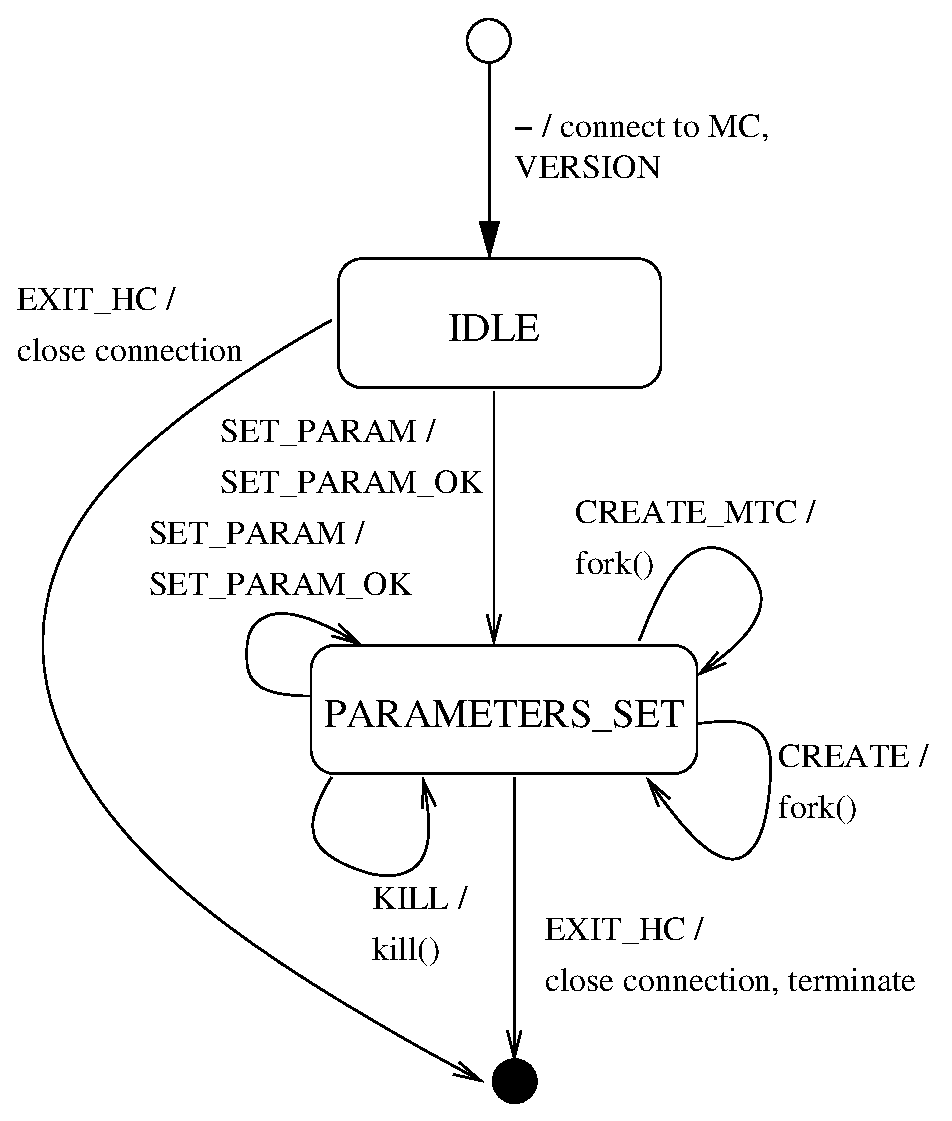
\includegraphics{state_mach_hc.eps}}}
\end{center}
\caption{\label{figure:state_mach_hc}State machine for HCs}
\end{figure}

\begin{figure}[!p]
\begin{center}
{\resizebox*{1 \columnwidth}{!}{\includegraphics{state_mach_hc_mc.eps}}}
\end{center}
\caption{\label{figure:state_mach_hc_mc}State machine for HCs as seen by the MC}
\end{figure}

\begin{figure}[!p]
\begin{center}
{\resizebox*{0.5 \columnwidth}{!}{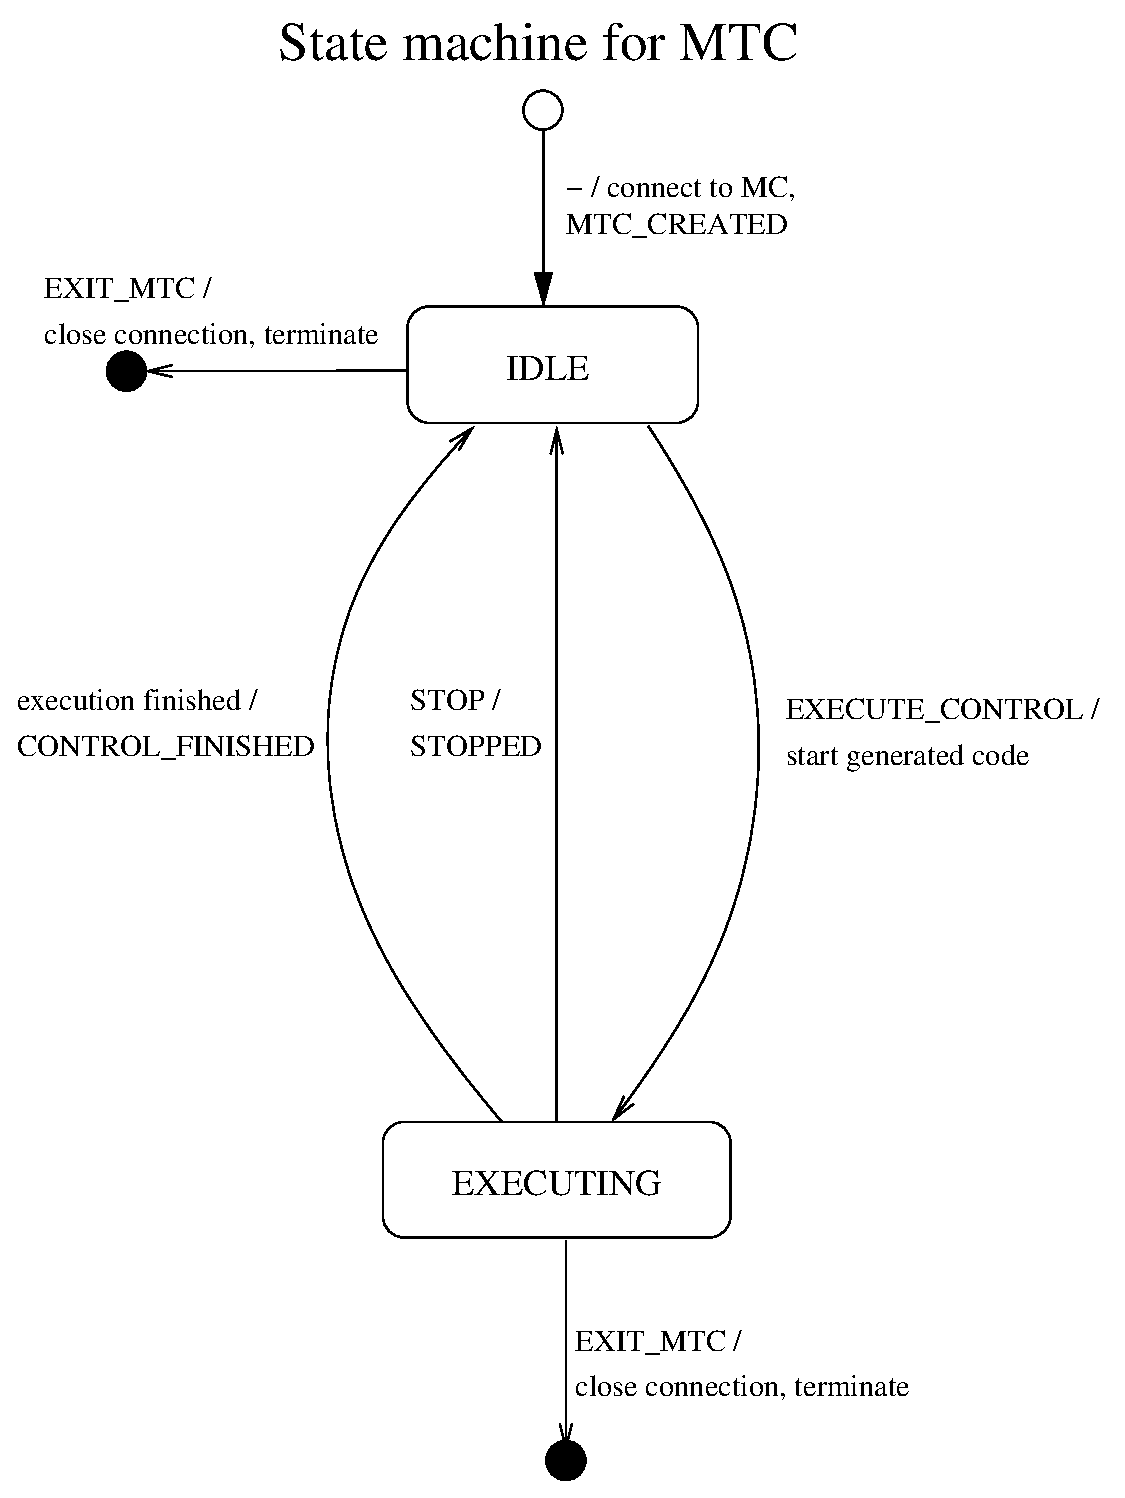
\includegraphics{state_mach_mtc.eps}}}
\end{center}
\caption{\label{figure:state_mach_mtc}State machine for the MTC}
\end{figure}

\begin{figure}[!p]
\begin{center}
{\resizebox*{1 \columnwidth}{!}{\includegraphics{state_mach_ptc_mc.eps}}}
\end{center}
\caption{\label{figure:state_mach_ptc_mc}State machine for PTCs as seen by the MC. States filled with grey colour and solid lines are used by both alive and non-alive PTCs. States with white background and dashed lines are used by alive PTCs only.}
\end{figure}

\begin{figure}[!p]
\begin{center}
{\resizebox*{1 \columnwidth}{!}{\includegraphics{state_mach_conn_endpoint.eps}}}
\end{center}
\caption{\label{figure:state_mach_conn_endpoint}State machine for port connection endpoints (the other endpoint is on a different component)}
\end{figure}

\begin{figure}[!p]
\begin{center}
{\resizebox*{\columnwidth}{!}{\includegraphics{state_mach_conn_mc.eps}}}
\end{center}
\caption{\label{figure:state_mach_conn_mc}State machine for port connections as seen by the MC}
\end{figure}

\begin{figure}[!p]
\begin{center}
{\resizebox*{1 \columnwidth}{!}{\includegraphics{state_mach_mapping_mc.eps}}}
\end{center}
\caption{\label{figure:state_mach_mapping_mc}State machine for port mappings as seen by the MC}
\end{figure}

\end{document}
